\clearpage



\appendix

\addcontentsline{toc}{chapter}{Appendix A\label{Normalization_example}}
\markright{Appendix A}
\begin{center}

\begin{center}{
\Huge \bf Appendix A}
\end{center}

\vspace{-1cm}
\section*{Normalization Example}
\end{center}


A practical example will be used in this appendix to show step by step the process of normalization and the derived recommendations for the orientation angles optimization from Chapter \ref{Chapter_1}. 


An area of $5 \mathrm{m^2}$ is given for PV cell deployment in Greenwich. There are $N$ PV cells to deploy. The energy conversion efficiency of all PV cells $\eta$ is set at 0.2 and the inclination angle of all PV cells $\gamma$ is set at $36^{\mathrm{o}}$ (optimal inclination angle for Greenwich (London, UK) in summer). The time step duration $\tau$ is set at 15min = $15\cdot60$s = 900s and the total number of time steps $T$ is set at 96. We assume that the BS is located near a school. Hence, the energy consumption $C^{\text{original}}(t)$ of the BS is 600000J=0.6MJ per 15 minutes during school hours, i.e., 8am-1pm ($t\in\{32,...,52\}$), and 300000J=0.3MJ per 15 minutes during the rest of the day, i.e., $t\in\{1,...,31\}$ or $t\in\{53,...,96\}$.



Among all orientation angle settings and among all time steps throughout the day, the peak energy generation occurs during noon when all PV cells are south-oriented in Greenwich. This is because Greenwich is located on the reference meridian of its time zone. This peak energy generation value $PEG$ is used to normalize the energy generation profiles of the PV cells as well as the energy consumption profile of the BS for convenience. This has the convenient effect that the normalized peak energy generation is exactly 1 unit of normalized energy as seen in Figure \ref{norm}.  The time step $t=\frac{T}{2}$ is noon. The peak energy generation value of all PV cells (south-oriented) at noon in this example is 552600J as follows:

\begin{align}
PEG = & G^{\text{original}}_{0^{\mathrm{o}},1}\big(\frac{T}{2}\big)= \sum_{n=1}^N G^{\text{original}}_{0_n^{\mathrm{o}},N}\big(\frac{T}{2}\big)= \sum_{n=1}^N I_{0_n^{\mathrm{o}}}\big(\frac{T}{2}\big)\cdot \eta \cdot \frac{A}{N} \cdot \tau=\\
&\sum_{n=1}^N 614 \cdot 0.2 \cdot \frac{5}{N}  \cdot 900 = 614 \cdot 0.2 \cdot 5  \cdot 900 =552600.
\end{align}

$614 \frac{\mathrm{W}}{\mathrm{m^2}}$ is obtained from the PVGIS database as seen in Figure \ref{normal2}. 

\begin{figure}[H]
	\centering
		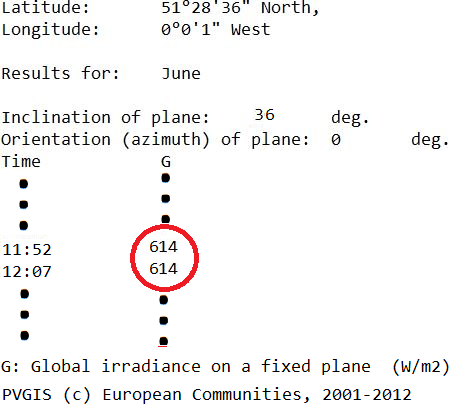
\includegraphics[width=0.5\columnwidth]{pictures/normal2}
\caption{PVGIS data sheet from \cite{PVGIS}. $\gamma$ is set at $36^{\mathrm{o}}$, $\theta$ is set at $0^{\mathrm{o}}$, month is set at June, and the location is Greenwich ($lat=51.4767^{\mathrm{o}}$ North, $lon=0.0003^{\mathrm{o}}$ West).\label{normal2}}
\end{figure}

Hence, $G_{\theta,N}(t)$ is the normalized energy generated by one PV cell (out of the $N$ PV cells) installed with orientation angle $\theta$ at time step $t$ and can be calculated by

\begin{equation}\label{eins}
G_{\theta,N}(t)=\frac{G_{\theta,N}^{\text{original}}(t)}{G^{\text{original}}_{0^{\mathrm{o}},1}\big(\frac{T}{2}\big)}=\frac{G_{\theta,N}^{\text{original}}(t)}{\textcolor{blue}{552600}}=\frac{I_{\theta}(t)}{I_{0^{\mathrm{o}}}\big(\frac{T}{2}\big)\cdot N}= \frac{I_{\theta}(t)}{\textcolor{green}{614\cdot N}}.
\end{equation}



\begin{figure}[H]
	\centering
		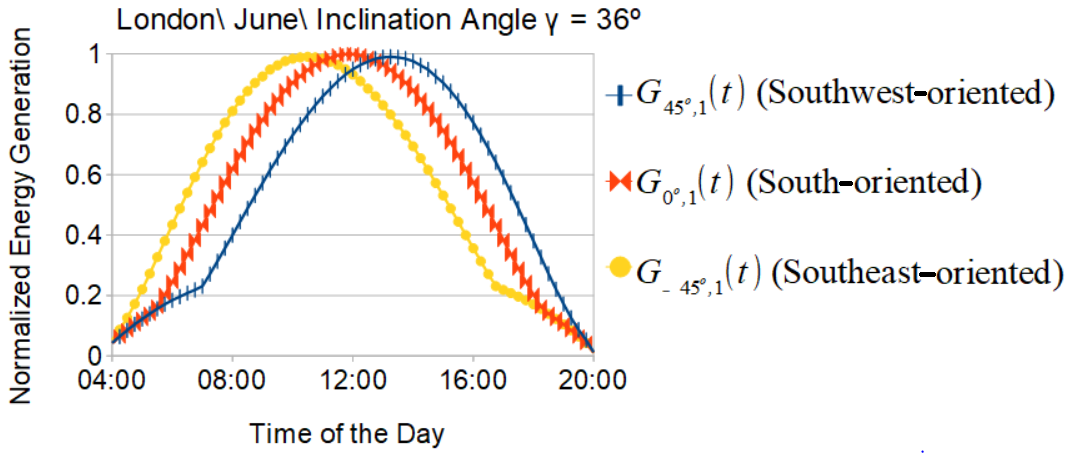
\includegraphics[width=1\columnwidth]{pictures/orien}
\caption{Normalized energy generation profiles of a southeast-oriented, south-oriented, and southwest-oriented PV cell. Each of the PV cells is covering the total surface area $A=5\mathrm{m^2}$. The south-oriented PV cell generates at noon the most energy among all orientation angle settings and among all time steps throughout the day. This normalized peak energy generation is exactly 1 unit of normalized energy.\label{norm}}
\end{figure}

Hence, $C(t)$ is the normalized energy consumption by the BS at time step $t$ and can be calculated by

\begin{equation}\label{zwei}
C(t)=\frac{C^{\text{original}}(t)}{G^{\text{original}}_{0^{\mathrm{o}},1}\big(\frac{T}{2}\big)}=\frac{C^{\text{original}}(t)}{\textcolor{blue}{552600}}.
\end{equation}

I want to point out, that the energy generation profiles as well as the energy consumption profile are normalized by the same value \textcolor{blue}{552600J}. But because the irradiance $I_{\theta}(t)$ value was calculated in Chapter \ref{Chapter_1}, the irradiance $I_{\theta}(t)$ has to be normalized by $\textcolor{green}{614\frac{\mathrm{W}}{\mathrm{m^2}}\cdot N}$ to achieve the same normalization, cf. (\ref{eins})-(\ref{zwei}). 


I want to point out, that the energy generation profiles as well as the energy consumption profile are normalized by the same value 552600J. This is because I want to keep the same relationship between the two types of profiles after the normalization. That means if the energy consumption at time step $t$ is double the amount of the energy generated by the PV cells at time step $t$ before the normalization, the same should be true after the normalization, i.e., the normalized energy consumption at time step $t$ is double the amount of the normalized energy generated by the PV cells at time step $t$. This can be proven mathematically by

\begin{equation}
\frac{C(t)}{G_{\theta,N}(t)}=\frac{\frac{C^{\text{original}}(t)}{552600}}{\frac{G_{\theta,N}^{\text{original}}(t)}{552600}}=\frac{C^{\text{original}}(t)}{G_{\theta,N}^{\text{original}}(t)}.
\end{equation}



Figure \ref{gggg}, and Figure \ref{gg} show the energy generation profile of one PV cell and the energy consumption profile of the BS before normalization, and after normalization for the given example, respectively. The energy generation profile of a south-oriented PV cell covering the total surface area ($A=5\mathrm{m^2}$) is depicted. The shapes of the two profiles are the same in both figures. The relationship between the energy generation profile and the energy consumption profile is the same in both figures. Only the description of the primary y-axis and secondary y-axis changes between the two figures. 

\begin{figure}[H]
	\centering
		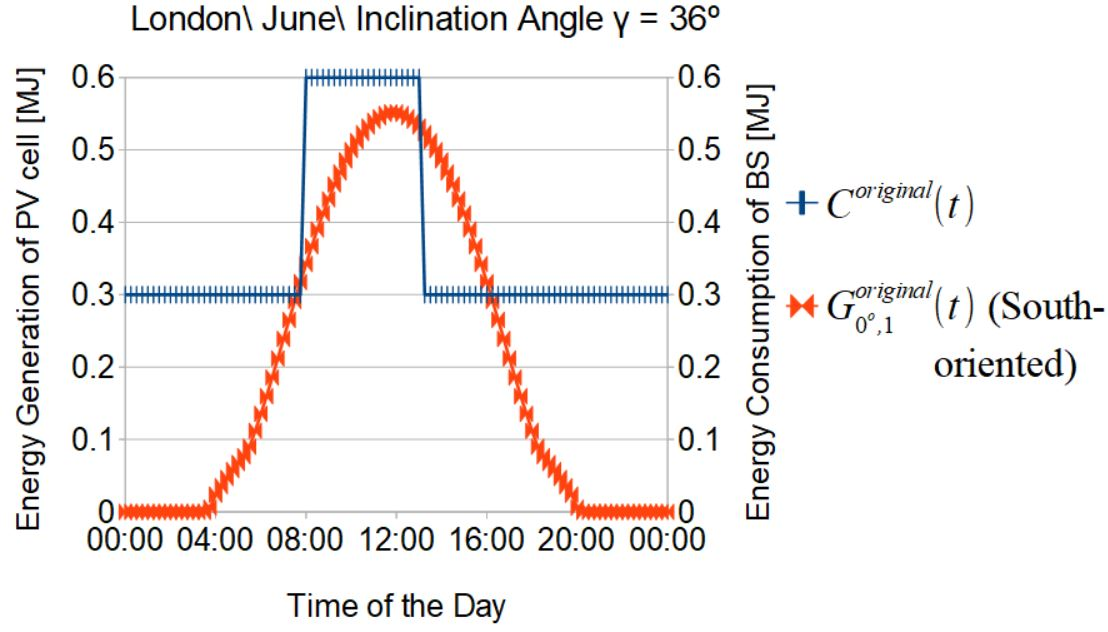
\includegraphics[width=1\columnwidth]{pictures/gggg}
\caption{Energy generation profile $G_{0^{\mathrm{o}},1}^{\text{original}}(t)$ and energy consumption profile $C^{\text{original}}(t)$ before normalization. \label{gggg}}
\end{figure}


\begin{figure}[H]
	\centering
		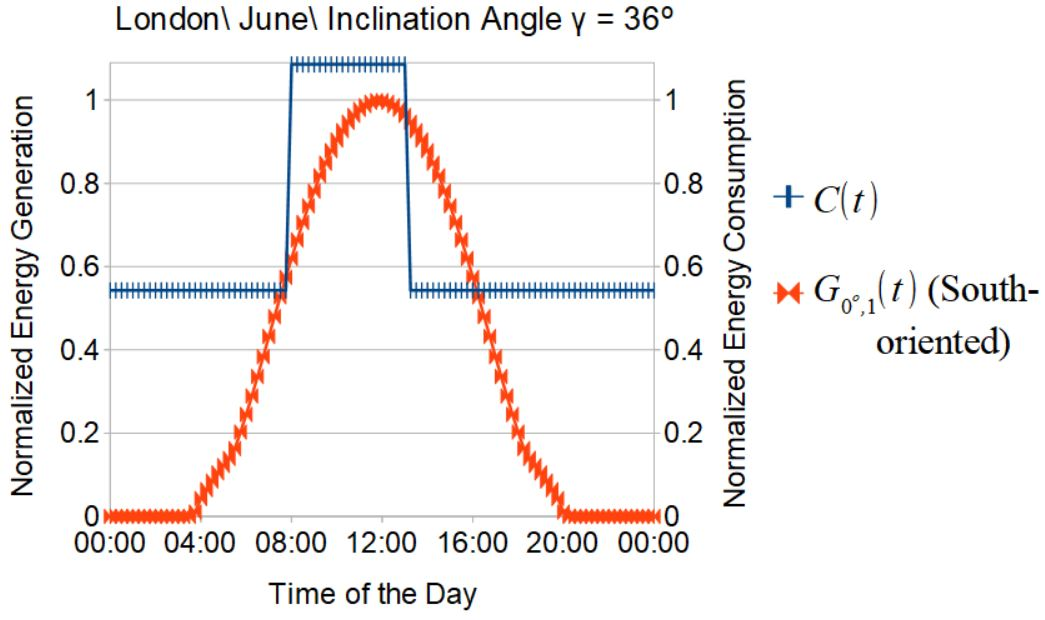
\includegraphics[width=1\columnwidth]{pictures/gg}
\caption{Energy generation profile $G_{0^{\mathrm{o}},1}(t)$ and energy consumption profile C(t) after normalization.\label{gg}}
\end{figure}


Figure \ref{gg} reveals that the energy consumption profile is similar to the business-area traffic load profile from Chapter \ref{Chapter_1} (one significant peak during sunrise and sunset). In addition, Figure \ref{gg} reveals that the energy generation is slightly smaller than the energy consumption, i.e., $G<C$. That means, the orientation angle optimization for this example will show a similar behavior as that of table cell (e) in Table \ref{table_1PV}, Table \ref{table_2PV}, and Table \ref{table_3PV}, if 1 PV cell, 2 PV cells, and 3 PV cells are deployed on the total surface area of $5\mathrm{m^2}$, respectively. 
The optimal solution in this example is to deploy one PV cell (or several PV cells) with the (same) optimized orientation angle on the total surface area of $5\mathrm{m^2}$. The optimal orientation angle will be slightly to the east because the energy consumption peak is slightly shifted to the morning hours. The exact value of the optimal orientation can be calculate with the method presented in Chapter \ref{Chapter_1}. 

\newpage 

\addcontentsline{toc}{chapter}{Appendix B}
\markright{Appendix B}


\begin{center}

  \begin{center}{
   \Huge \bf Appendix B}
  \end{center}

\vspace{-1cm}
\section*{MATLAB Source Code of Chapter \ref{Chapter_1} \cite{DOBEN_GITHUB}}
\end{center}

		\section*{Main File:}
		\scriptsize
		\lstinputlisting[language=Matlab]{Matlab_code/MAIN_FILE_orientation_angle_optimization.m}
		
		\section*{Ground-reflected Irradiance:}
		\lstinputlisting[language=Matlab]{Matlab_code/I_ground.m}
		
		\section*{Direct-beam Irradiance:}
		\lstinputlisting[language=Matlab]{Matlab_code/I_beam.m}
				
		\section*{Sky-diffuse Irradiance:}
		\lstinputlisting[language=Matlab]{Matlab_code/I_diffuse.m}

	  \section*{Normalized Energy Drawn from the Main Grid:}
		\lstinputlisting[language=Matlab]{Matlab_code/normalized_energy_drawn_from_the_main_grid.m}
		
		\section*{Output (1 PV Cell):}
		\lstinputlisting[language=Matlab]{Matlab_code/print_1D_graph.m}
		
		\section*{Output (2 PV Cells):}
		\lstinputlisting[language=Matlab]{Matlab_code/print_2D_graph.m}
		
		\section*{Output (3 PV Cells):}
		\lstinputlisting[language=Matlab]{Matlab_code/print_3D_graph.m}
		
		\section*{Input File (Load Profiles):}
		\lstinputlisting[language=Matlab]{Matlab_code/load_profiles.txt}
		
		\section*{Input File (PVGIS \cite{PVGIS}):}
		\lstinputlisting[language=Matlab]{Matlab_code/jun_dailyrad512836N_000001W_0deg_0deg.txt}
